% ---------------------------------------------------------------
\subsection{Extra Task ET1 -- Fractional sensitivity of the heat flux to the inputs}
\label{sec:et1}

\paragraph{Method.}
Program \code{P2\_ET1.ipynb} uses the best-fit constants of Task~2.3 and follows steps 1--3 of the
statement for three typical sets of inputs: S1 (earth gravity, $\dTsat_1=40$\,\textdegree C, $g_1=9.8$~m/s$^2$,
$\gamma_1=1.79$, $P_1=5.5$~kPa), S2 (the same at $0.01\,\gen$) and S3 ($2\,\gen$, 9.5~kPa, 35\,\textdegree C).
\begin{enumerate}[label=\arabic*)]
  \item $\qpp_1$ is computed with Eq.~(1.5) for the typical inputs;
  \item one input at a time is changed: the superheat by $\Delta\dTsat=2$\,\textdegree C, as in the statement, and
        $g$, $\gamma$, $P$ by $5\,\%$ (the same relative step as 2\,\textdegree C at 40\,\textdegree C), giving $\qpp_2$;
  \item the fractional change ratio is
        $S_x=\dfrac{\Delta\qpp/\qpp_1}{\Delta x/x_1}=\dfrac{(\qpp_2-\qpp_1)\,x_1}{\Delta x\,\qpp_1}$.
\end{enumerate}
For comparison, the limit $\Delta x\to0$ gives analytical values: $S_{T}=n_2$,
$S_g=n_3\,g/(g+n_4\gen\gamma)$, $S_\gamma=n_3\,n_4\gen\gamma/(g+n_4\gen\gamma)$ and $S_P=n_5$.

\begin{table}[H]
\centering\small
\caption{ET1: fractional change ratios (finite steps). The analytical limit $\Delta x\to0$ is given in
parentheses.}
\label{tab:et1}
\fittable{et1_sens}
\end{table}

\begin{figure}[H]
\centering
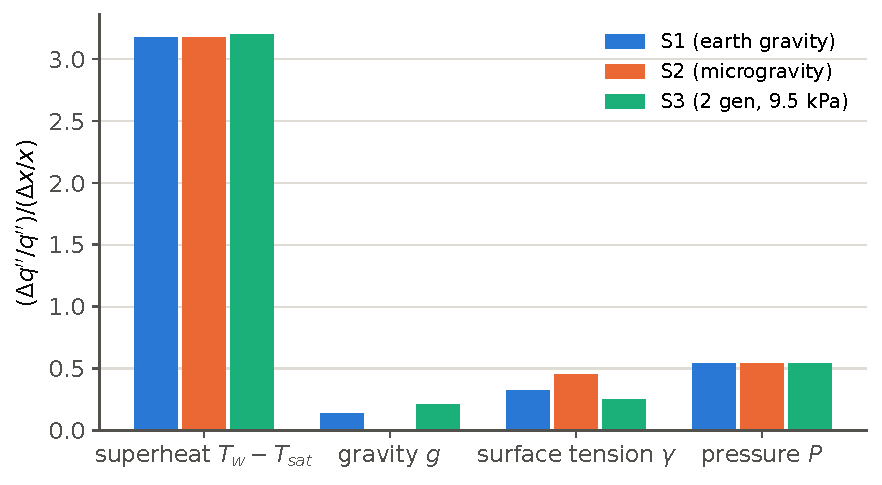
\includegraphics[width=0.62\linewidth]{figures/et1_sensitivity.pdf}
\caption{ET1: fractional sensitivity of the predicted heat flux to each input for the three typical states.}
\label{fig:et1}
\end{figure}

\paragraph{Results (Table~\ref{tab:et1}, Fig.~\ref{fig:et1}).}
\begin{itemize}
  \item \textbf{The heat flux is by far most sensitive to the superheat}: $S_T=\EtOneSdT$. A $1\,\%$ error
        on $T_w-T_{sat}$ gives a $3\,\%$ error on $\qpp$. The finite-step value is a little higher than
        $n_2=3.02$ because $(1.05)^{3.02}-1=0.159$ is more than $3.02\times0.05$ (non-linearity of the
        power law).
  \item The sensitivity to pressure is the same in all states ($S_P\approx n_5\approx0.54$).
  \item The sensitivities to $g$ and $\gamma$ depend on the state, because the two effects share the
        effective gravity $g+n_4\gen\gamma$. At earth gravity, $S_g=\EtOneSg$ and $S_\gamma=\EtOneSgam$.
        In microgravity, $S_g=\EtOneSgLow$: the gravity level no longer matters, and $S_\gamma$ increases
        to \EtOneSgamLow\ because Marangoni flow provides almost all the liquid supply.
\end{itemize}

\paragraph{Limiting fractional inaccuracy of the inputs for $|\Delta\qpp/\qpp|<0.15$.}
To first order,
$\Delta\qpp/\qpp=S_T\,\varepsilon_T+S_g\,\varepsilon_g+S_\gamma\,\varepsilon_\gamma+S_P\,\varepsilon_P$, where
$\varepsilon_x=\Delta x/x$. Three estimates are given in Table~\ref{tab:et1lim}:
(i) only one input is inaccurate, $\varepsilon_x<0.15/|S_x|$;
(ii) all inputs have the same inaccuracy $\varepsilon$ and the errors add up in the worst direction,
$\varepsilon<0.15/\sum|S_x|$;
(iii) the same $\varepsilon$, but independent random errors combined as a root-sum-square,
$\varepsilon<0.15/\sqrt{\sum S_x^2}$.

\begin{table}[H]
\centering\small
\caption{ET1: limiting fractional inaccuracy of the inputs for a fractional inaccuracy of the predicted
heat flux below 0.15. Last column: corresponding superheat uncertainty for case (ii).}
\label{tab:et1lim}
\fittable{et1_limits}
\end{table}

\textbf{Conclusion.} The superheat must be known to about $\EtOneSingle\,\%$ if it is the only
inaccurate input ($\pm\EtOneSingleC$\,\textdegree C at 40\,\textdegree C). If all inputs have the same fractional inaccuracy
and the errors add up, they must all be known to about $\EtOneWorst\,\%$ ($\pm\EtOneWorstC$\,\textdegree C on the
superheat). With random, independent errors the limit is about $\EtOneRss\,\%$. These estimates were
checked with the full non-linear model: changing all inputs by $3.6\,\%$ in the unfavourable direction
gives $\Delta\qpp/\qpp=\EtOneCheck\,\%$. Since the superheat dominates, a practical error budget is, for
example, superheat $\pm3\,\%$ ($\pm1.2$\,\textdegree C), pressure $\pm3\,\%$, $\gamma$ $\pm5\,\%$ and $g$ $\pm10\,\%$.
Even in the worst case, this gives $3.18(0.03)+0.54(0.03)+0.32(0.05)+0.13(0.10)=0.14<0.15$.
\textbf{The accuracy of the predicted heat flux is therefore limited mainly by the accuracy of the wall
superheat measurement.} An uncertainty of $\pm2$\,\textdegree C, which is not unusual for a wall temperature
measurement in a flight experiment, would by itself use up the whole $15\,\%$ budget.

% ---------------------------------------------------------------
\subsection{Extra Task ET2 -- Inverse relation for the superheat}
\label{sec:et2}

\paragraph{Method.}
Program \code{P2\_ET2.ipynb} reorganises the 77 data points of Task~2.3 as
$[T_w-T_{sat},\ \qpp,\ g,\ \gamma,\ P]$, so that $\qpp$, $g$, $\gamma$, $P$ are the inputs and the
superheat is the output. It then fits Eq.~(ET2.1),
$\dTsat=\nh1(\qpp)^{\nh2}(g+\nh4\gen\gamma)^{\nh3}P^{\nh5}$, with a copy of the Task~2.3 GA (error
normalised by $|\ln\dTsat|$). Three sets of initial guesses were used: (I) the values implied by Task~2.3,
(II) $(10,\,0.5,\,-0.1,\,1,\,-0.1)$ and (III) $(40,\,0.25,\,-0.25,\,2,\,-0.3)$, each with 3 seeds and the
same refinement as in Task~2.3. The best GA fit is
$\dTsat=20.27\,(\qpp)^{0.3074}(g+1.308\,\gen\gamma)^{-0.1455}P^{-0.1485}$ with $\Ferrmean=\EtTwoGaF$.
The superheat is predicted with an rms deviation of 1.8\,\textdegree C (mean absolute deviation $3\,\%$, about one
third of the deviation on $\qpp$, consistent with $n_2\approx3$).

\begin{table}[H]
\centering\small
\caption{ET2: best-fit $\hat n_i$ from the GA fit of (ET2.1), compared with the values computed from
the best-fit $n_i$ of Task~2.3 with the relations of the statement. Right: the same comparison between the
exact minima of the two error functions (deterministic check). Difference $=(\text{fit}-\text{implied})/|\text{implied}|$;
for the negative exponents $\hat n_3$ and $\hat n_5$, a positive difference means a smaller magnitude.}
\label{tab:et2}
\fittable{et2_table}
\end{table}

\paragraph{Do the two sets of $\hat n_i$ agree?}
They are \emph{close but not identical} (Table~\ref{tab:et2}). The differences are typically
$3$--$10\,\%$: $\nh1$ $\EtTwoDiffOne\,\%$, $\nh2$ $\EtTwoDiffTwo\,\%$, $\nh3$ $\EtTwoDiffThree\,\%$, $\nh4$
$\EtTwoDiffFour\,\%$, and up to $\EtTwoDiffFive\,\%$ for the weakly determined pressure exponent $\nh5$. The
only systematic difference is on $\nh2$: the direct fit of the superheat gives an exponent on $\qpp$
about $7$--$8\,\%$ smaller than $1/n_2$. The same differences appear between the exact minima of the two
error functions (right part of the table), so they are not caused by the GA. The implied values also give a
larger error for (ET2.1) ($\EtTwoImpF$ vs.\ $\EtTwoGaF$), which shows that the two fits really are different
optima.

\paragraph{Is the noise in the data responsible?}
Yes. Fitting $y$ versus $x$ and $x$ versus $y$ gives two slopes whose product is $r^2<1$ when the data
scatter, so the inverse exponent $\nh2$ must come out smaller than $1/n_2$. To check this quantitatively,
I made synthetic data with Eq.~(1.5) and the Task~2.3 constants, at the 77 measured conditions
(Table~\ref{tab:et2noise}):
\begin{itemize}
  \item[(a)] \textbf{Noise-free data}: the GA fit of (ET2.1) ($\Ferrmean=\EtTwoNoiseFreeF$) recovers the
        implied values to within $0.03\,\%$. The method and the relations of the statement are therefore
        exact when there is no noise.
  \item[(b)] \textbf{Scatter added to $\qpp$} (log-normal, standard deviation $\EtTwoSigma$, equal to the
        rms residual of the Task~2.3 fit; 30 realisations): the inverse fit gives $\nh2$ $7\pm2\,\%$ below
        $1/n_2$, exactly the difference found with the measured data. The other exponents scatter by
        $\pm5$--$10\,\%$ from one realisation to the next, which is the size of the differences in
        Table~\ref{tab:et2}.
  \item[(c)] \textbf{The same scatter put on the superheat instead} gives the same result. Which variable
        carries the noise only changes which of the two fits is unbiased, not the fact that they disagree.
\end{itemize}

\begin{table}[H]
\centering\small
\caption{ET2: percentage difference between the inverse fit and the values implied by the forward fit,
for the measured data and for synthetic data generated with Eq.~(1.5) (mean $\pm$ standard deviation over
30 noise realisations).}
\label{tab:et2noise}
\fittable{et2_noise}
\end{table}

\textbf{Conclusion.} The differences between the directly fitted $\hat n_i$ and those computed from
the Task~2.3 constants ($\approx2$--$17\,\%$, typically $5$--$10\,\%$) come from the scatter in the data:
it produces a systematic $\approx7\,\%$ reduction of $\nh2$ (regression dilution) and random differences of
the other constants of the same size as their run-to-run variability. The two relations are equally valid
descriptions of the data. Each one should be used in the direction in which it was fitted: the heat flux
from the superheat with Eq.~(1.5), and the superheat from the heat flux with Eq.~(ET2.1).

\begin{figure}[H]
\centering
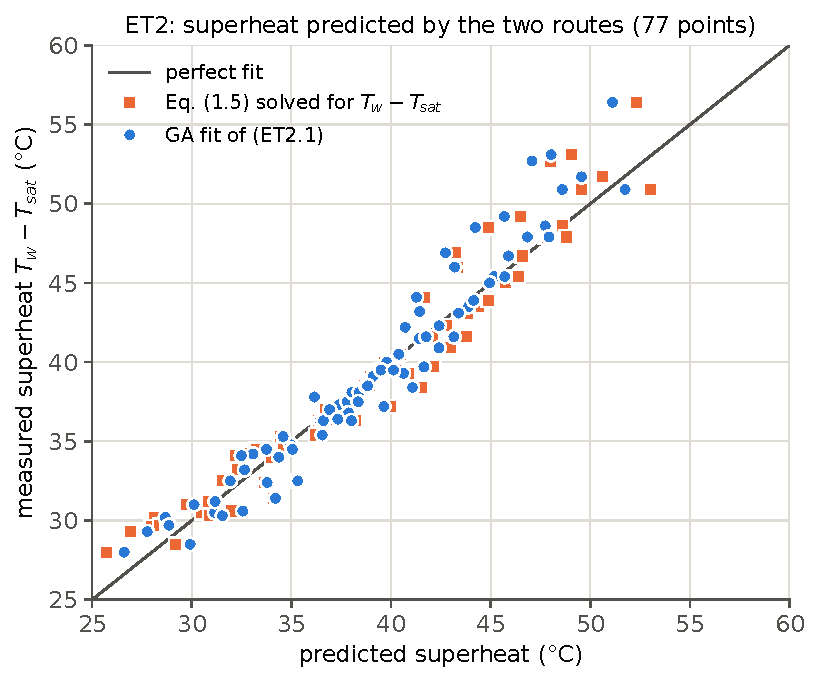
\includegraphics[width=0.55\linewidth]{figures/et2_parity.pdf}
\caption{ET2: measured superheat versus the superheat predicted by the GA fit of (ET2.1) and by Eq.~(1.5)
solved for $T_w-T_{sat}$.}
\label{fig:et2}
\end{figure}
